\section{Future Work}


\subsection{Improve Robustness}
In this paper we have made many simplifications to the problem space just to make the placer easier to implement.
For example, our placer in its current state does not take advantage of \texttt{SLICEL}/\texttt{SLICEM} homogeneity and simply maps all SLICE \texttt{SiteInst}s onto \texttt{SLICEL}s. 
Recall that the SLICE Sites in Xilinx FPGAs typically come in a 75-25\% split between \texttt{SLICEL}s and \texttt{SLICEM}s. 
This means that we have rendered about 25\% of the CLB fabric unusable which will inevitably hurt wirelength minimization during placement since the \texttt{SiteInst}s must be spread over a larger area. 
Enabling \texttt{SLICEL}-\texttt{SLICEM} homogeneity can lead do greater logic density and consequently less total HPWL, but can make the packing process more complex and may contribute to higher routing congestion.

We can also add packing support for other Xilinx primitives such as the shift-register primitive \texttt{SRLx}, distributed RAM primitives \texttt{RAMSx}, or even \texttt{LATCH} primitives as discussed in \ref{sec:7_series}.
Adding support for additional primitives and macros will allow our placer to handle a wider range of HDL designs and will require deeper consideration of hardware constraints to ensure robustness.

In its current state, the prepacker and packer struggle to handle signals larger than 24-bits, especially when involved in DSP functions like addition and multiplication. 
In such designs, the Vivado synthesizer may synthesize long \texttt{CARRY4} chains with particular \texttt{EDIFHierPortInst} configurations that are currently not handled by our packer and eventually to failures in the subsequent routing stage.
Further work is required to resolve these constraints in the packer.


\subsection{Variations on Packing}
Our current placer follows a \texttt{Site}-centric approach that resembles that of Xilinx ISE, which is the predecessor to the Vivado design suite that was primarily used in the 90s and 2000s.
The more modern Vivado now performs BEL-centric placement without necessarily locking \texttt{Cell}s into \texttt{Site}s, allowing for a higher granularity of movement of \texttt{Cell}s. 
Enabling BEL-centric movement as opposed to Site-centric movement in our placer can improve HPWL minimization, but will add much more complexity to the packing and placement process to ensure robustness with respect to hardware constraints.

There is also no rule saying we must pack \texttt{Cells} into \texttt{SiteInst}s before placement or that we follow a strict prepacking-packing-placement flow. 
Future work can 
{
    \centering
    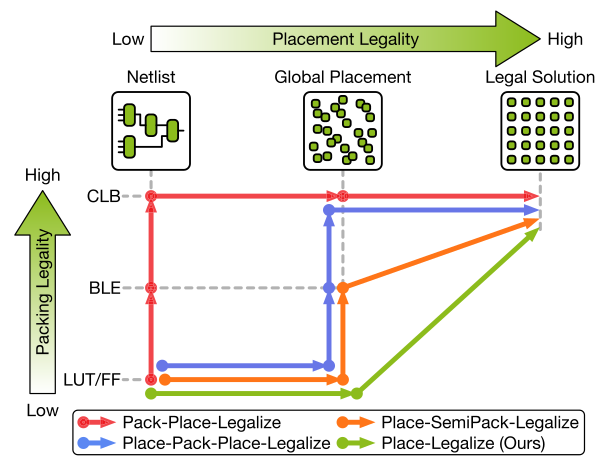
\includegraphics[width=\columnwidth]{figures/future_work/legalization.png}
    \captionof{figure}{Representative FPGA placement and packing flows. Figure taken from Wuxi et al. (2019), page 1 \cite{ExplicitPacking}}
}
\vspace{0.25cm}

\subsection{Add Hard Macro Support}

\subsection{Improvements to SA}

\subsection{Force-Directed and Analytical Placement}




